\section{RESCUER}
    \subsection{Home}

        \begin{figure}[H] \noindent \centering
            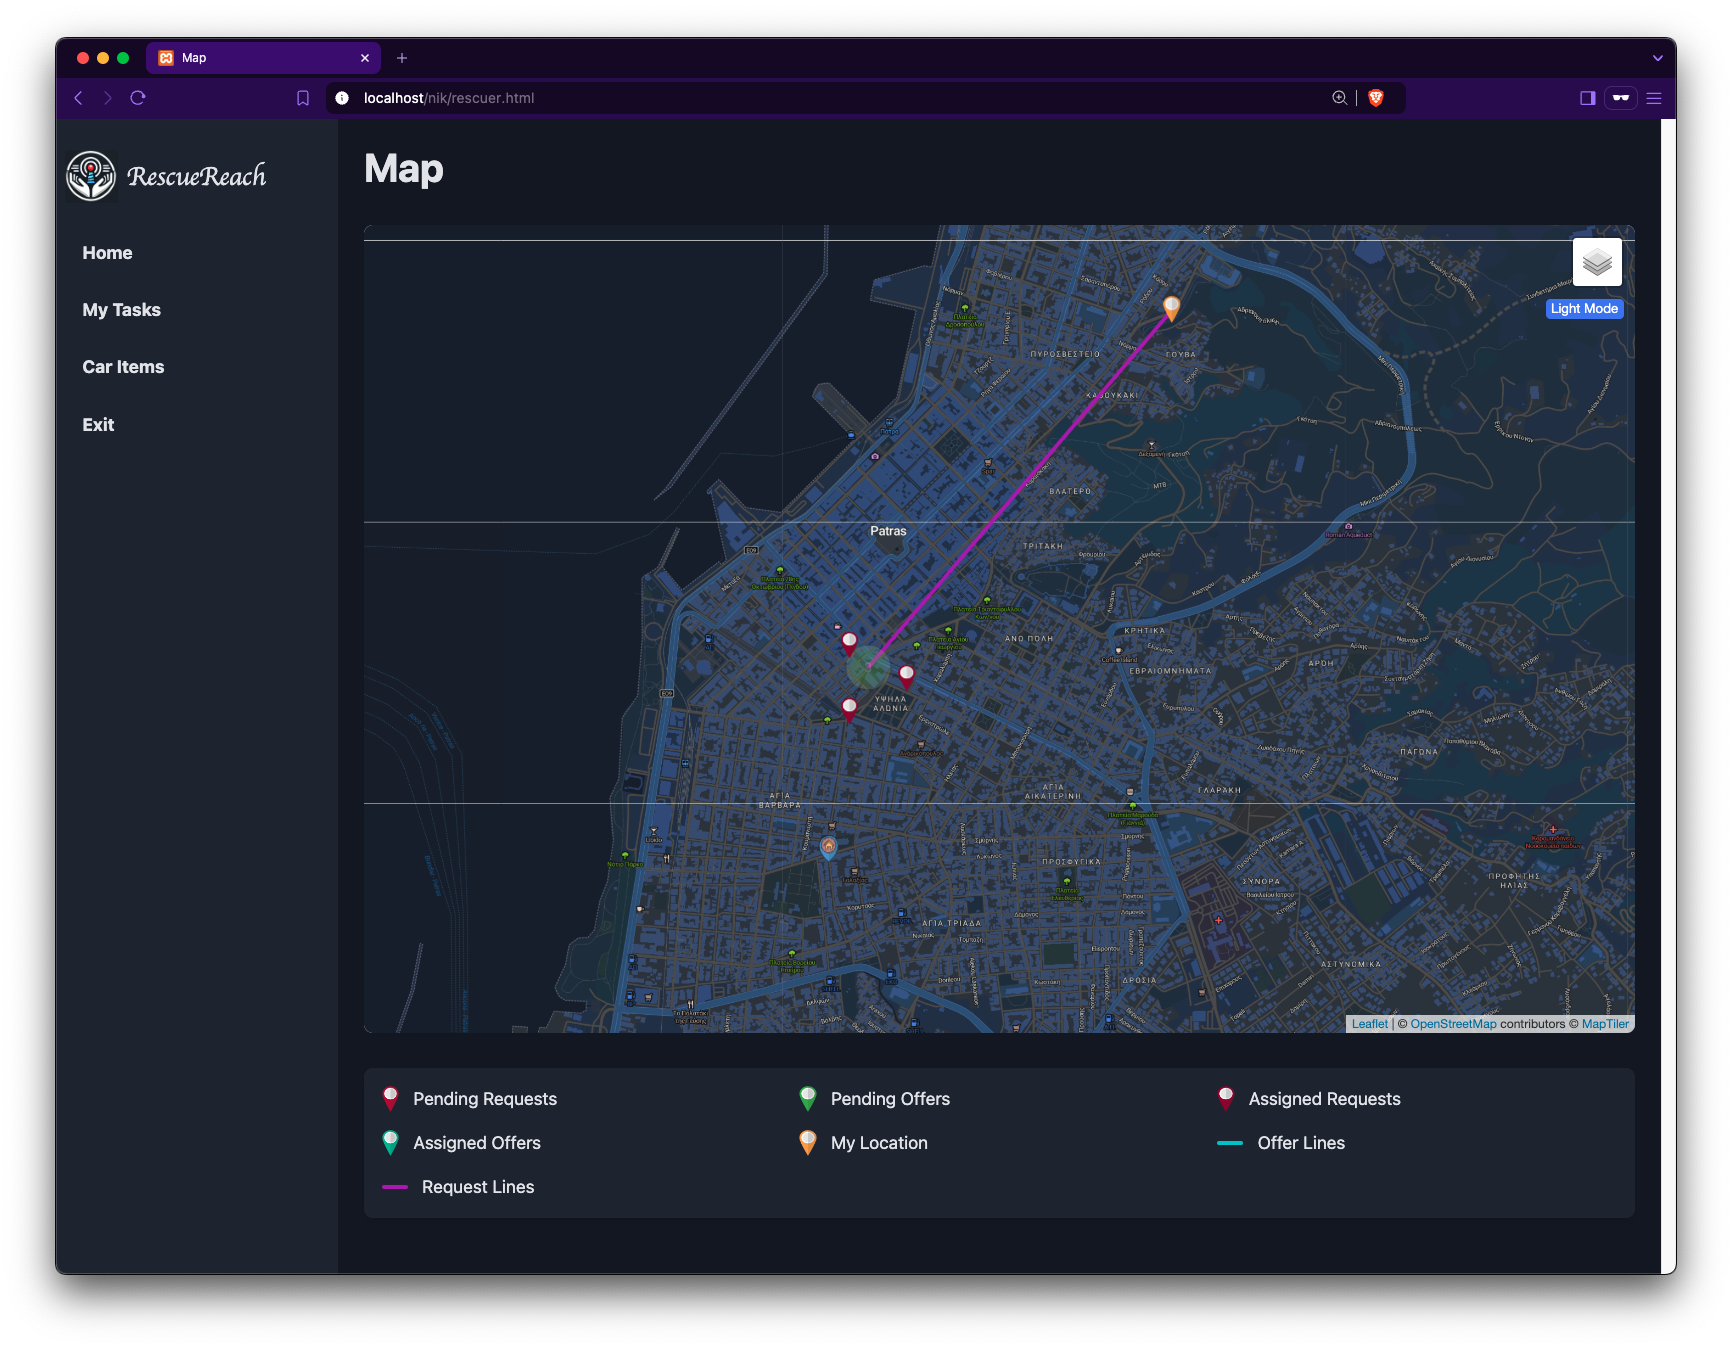
\includegraphics[width=0.8\textwidth]{img/rescuer-map}
            \caption{Αρχική σελίδα rescuer}
        \end{figure}

        Η αρχική σελίδα του διασώστη περιλαμβάνει το χάρτη της πόλης, με τα markers που αντιστοιχούν στα requests και τα offers των πολιτών.
        Ο rescuer δεν μπορεί να δει τους υπόλοιπους rescuers.
        Αυτό επιτυγχάνεται μέσω της \c{logged\_user} σταθεράς, που απομονώνει τον συγκεκριμένο χρήστη από τα δεδομένα που επιστρέφονται από τη βάση δεδομένων.
        Η διαδικασία εμφάνισης των markers είναι παρόμοια όπως στη σελίδα του admin.

        \begin{figure}[H] \noindent \centering
            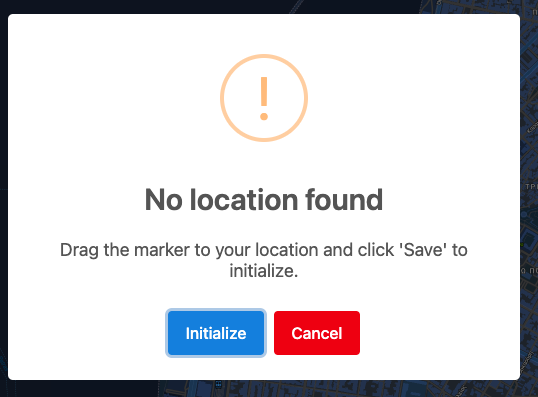
\includegraphics[width=0.4\textwidth]{img/rescuer-no_location}
            \caption{Αρχικοποίηση rescuer}
        \end{figure}

        Μια διαφορά που προκύπτει στην \c{fetchRescuerLocation()} είναι κατά την αρχικοποίηση της τοποθεσίας του διασώστη μετά την εγγραφή του από τον admin.

        \begin{figure}[H] \noindent \centering
            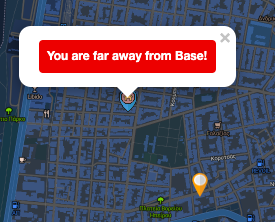
\includegraphics[width=0.3\textwidth]{img/rescuer-marker1}
            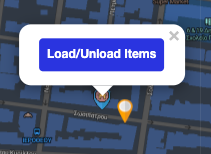
\includegraphics[width=0.3\textwidth]{img/rescuer-marker2}
            \caption{Ο διασώστης πρέπει να είναι σε ακτίνα 50m από τη βάση}
        \end{figure}

        Η \c{baseProximity()} ελέγχει την απόσταση του διασώστη από τη βάση και ανάλογα τροποποιεί το συννεφάκι της βάσης.
        Η \c{displayLines()} χρησιμοποιεί τις συντεταγμένες του διασώστη και των πολιτών και δημιουργεί γραμμές (\c{L.polyline}) μεταξύ τους.
        Τέλος η \c{takeTask()} ελέγχει με AJAX request στην \c{takeTask.php} πόσα tasks έχουν ήδη επιλεγεί από τους διασώστες, και αν είναι πάνω από 4, δεν επιτρέπει την επιλογή ενός νέου.